\subsection{Revisão Teórica}

Como já mencionado a reação base para todo o processo de produção do sabão é a saponificação. Entrando mais em detalhes agora, tal reação ocorre entre uma base forte, normalmente hidróxido de sódio (NaOH) ou de potássio (KOH), e triglicerídeos para formar sais de ácido graxo (sabão, produto principal) e glicerol (coproduto) \cite{neto2011trabalhando}, destacada na Figura~\ref{fig:reacao_saponificacao}.

\begin{figure}[H]
    \centering
    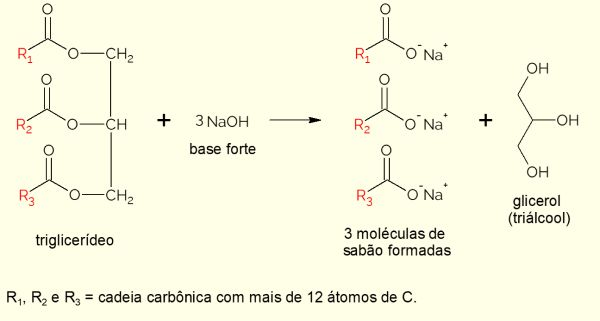
\includegraphics[width=0.7\textwidth]{src/fig/reacao_sap.jpg}
    \caption{Reação de saponificação \cite{santos2021saponificacao}}
    \label{fig:reacao_saponificacao}
\end{figure}

As rotas tecnológicas de produção de sabão envolvem diferentes métodos e processos definidos pelas condições operacionais e pelos objetivos de cada aplicação. A escolha da rota influencia diretamente variáveis como o tempo de processo, o consumo energético, a estabilidade do produto e a compatibilidade com diferentes matérias-primas e aditivos \cite{warra2010cold}. De modo geral, as principais rotas de produção podem ser classificadas em: saponificação a quente, saponificação a frio e \textit{fat splitting}.

\subsubsection{Saponificação a quente}

A saponificação a quente consiste no processo direto de reação entre triglicerídeos e uma base forte, como NaOH ou KOH, sob aquecimento controlado, com temperaturas tipicamente entre 60 e 100~°C. O calor aplicado acelera a quebra das ligações éster dos triglicerídeos, favorecendo a formação rápida e eficiente dos sais de ácidos graxos (sabão) e do coproduto glicerol.

Por se tratar de uma rota direta, em que a massa é moldada ao final da reação, ela dispensa a etapa de \textit{salting-out}, ou separação por adição de sal. Ao prescindir dessa separação, o processo a quente direto mantém o glicerol retido no produto final \cite{warra2010cold}.

A principal vantagem dessa rota é a rápida obtenção do produto. Ao final da etapa reacional, o sabão já está essencialmente saponificado, exigindo apenas um breve período de estabilização de três a cinco dias. Isso aumenta a produtividade e o controle sobre o término da reação, tornando a rota preferida em aplicações de pequena e média escala industrial. Como contrapartida, o aquecimento implica maior consumo energético e exige atenção ao controle térmico, pois temperaturas excessivas podem degradar compostos sensíveis ao calor, como fragrâncias e alguns aditivos funcionais \cite{alum2024saponification}.

\subsubsection{Saponificação a frio}

A saponificação a frio é a rota predominante na produção artesanal e cosmética de sabão. Assim como na rota a quente, consiste na saponificação direta de triglicerídeos com uma base forte, como o hidróxido de sódio, sem aquecimento intenso — empregando-se, no máximo, um aquecimento brando dos óleos antes da mistura com a solução alcalina \cite{warra2010cold}. A mistura deve permanecer sob agitação até atingir o ponto conhecido como \textit{trace}, estágio em que a viscosidade aumenta devido ao início da formação dos sais de ácidos graxos. Em seguida, o sabão é moldado e mantido em repouso durante o período de cura. Após a homogeneização sob agitação, eventuais aditivos sensíveis, como perfumes, são incorporados na etapa final, e a mistura é vertida em moldes, onde o sabão endurece por secagem ao ar \cite{warra2010cold}. 

O período de cura, que pode variar entre quatro e seis semanas conforme o tipo de óleo utilizado, constitui uma etapa de maturação na qual a saponificação é finalizada — visto que ainda restam grandes quantidades de triglicerídeos não reagidos. Essa etapa também é responsável pela evaporação parcial da água, ajustando a consistência e a pureza do sabão de acordo com as propriedades desejadas \cite{alum2024saponification}. 

Assim como na rota a quente direta, a saponificação a frio também dispensa o \textit{salting-out}, de modo que o glicerol é retido no produto e o sabão preserva a coloração do óleo de origem \cite{warra2010cold}. Para reduzir a alcalinidade residual e a agressividade do produto causadas pelo excesso de hidróxido de sódio, costuma-se empregar um excesso de gordura na formulação, técnica conhecida como \textit{superfatting} \cite{warra2010cold}. A principal vantagem dessa rota é a simplicidade operacional e a melhor preservação de compostos sensíveis ao calor; em contrapartida, a ausência de aquecimento torna a reação mais lenta, exigindo maior tempo para a estabilização do produto \cite{alum2024saponification}.

\subsubsection{\textit{Fat Splitting}}

O \textit{fat splitting} (hidrólise de gorduras) é uma rota industrial em que os triglicerídeos reagem diretamente com água, geralmente sob alta temperatura e pressão, sendo decompostos em ácidos graxos livres e glicerol. Em uma etapa posterior, esses ácidos graxos são neutralizados com uma base, como NaOH ou KOH, produzindo os sais de ácidos graxos que constituem o sabão. O diferencial dessa rota está justamente na separação entre a hidrólise e a neutralização: ao isolar os ácidos graxos antes da saponificação, obtém-se maior controle sobre a composição da matéria-prima e uma separação eficiente entre o produto e o coproduto glicerol, razão pela qual é amplamente empregada na fabricação de sabão em escala industrial \cite{sonntag1979fat}.

Atualmente, a tecnologia predominante dessa rota é o processo contínuo Colgate-Emery, que opera em contracorrente no interior de uma torre vertical de aço inoxidável: a água escoa de forma ascendente, enquanto os óleos e gorduras descem em sentido oposto. O sistema trabalha tipicamente a temperaturas de 250 a 260~°C e pressões de 45 a 55~bar, com tempo de residência de duas a três horas e conversão de até 99\%. Os ácidos graxos resultantes da hidrólise são recolhidos no topo da coluna, purificados por destilação e, então, neutralizados com a base para formar o sabão. Já a glicerina é obtida na base da torre, na forma de solução aquosa que posteriormente passa por um processo de concentração, por se tratar de um coproduto de alto valor agregado \cite{sonntag1979fat}.

% TODO: adicionar uma imagem do diagrama da rota